Un primer acercamiento a esta metodolog\'ia ser\'ia con una m\'aquina de 
 Turing que tiene por configuraci\'on inicial una cinta infinita
 con la entrada e infinitas cintas auxiliares vac\'ias, al leer
 un car\'acter en la cinta de entrada se copia dicho car\'acter a la primer 
 cinta auxiliar avanzando de posici\'on tanto en la cinta de entrada como 
 en la cinta auxiliar, posteriormente se lee el siguiente car\'acter y 
 nuevamente se copia en esta primer cinta; se prosigue de la misma forma 
 hasta encontrar alg\'un car\'acter existente en la cinta auxiliar, en 
 este caso, se verifica si este car\'acter es el primero de la cinta
 auxiliar, en caso de no serlo, se copia a la siguiente cinta auxiliar, 
 repitiendo el proceso de lectura de la entrada y copia en la auxiliar. 
 Para el caso de que sea el mismo car\'acter de la primer cinta auxiliar, 
 se contin\'ua la lectura de la cinta de entrada verificando que cada car\'acter 
 sea igual tanto en la cinta de entrada como en la primer cinta; si alg\'un 
 car\'acter llega a ser diferente se copiar\'a desde el inicio hasta el 
 car\'acter actual en la siguiente cinta vac\'ia.

  
En la figura \ref{fig:alg01} se puede apreciar un ejemplo de la simulaci\'on de 
 la m\'aquina de Turing explicada anteriormente. Considerando como cadena de 
 ejemplo ``ABCDEABDEABXGRWACE'', ``ABCDE'' se escriben en la primer cinta 
 auxiliar, al leer el car\'acter ``A'', se identifica que ya existe en esta 
 cinta y es el primer car\'acter, por lo que se empieza a verificar que sean
 los mismos caracteres, los de la cinta de entrada que los de la cinta 
 auxiliar, al llegar al car\'acter ``D'' de la cinta de entrada, ve observa 
 que el de la cinta auxiliar es una ``C'', dado que son diferentes se copia 
 el contenido anterior a esta diferencia de la cinta auxiliar a la siguiente 
 cinta auxiliar, continuando con la lectura de la cinta de entrada se termina 
 de escribir en la segunda cinta auxiliar la cadena ``ABDE'', ya que el 
 siguiente car\'acter es otra ``A'' se vuelve a verificar desde el inicio de 
 la cadena. Repitiendo el proceso se obtiene una tercer cadena (``ABXGRW'') 
 y una cuarta (``ACE'').
  
\begin{figure}[h]
\centering
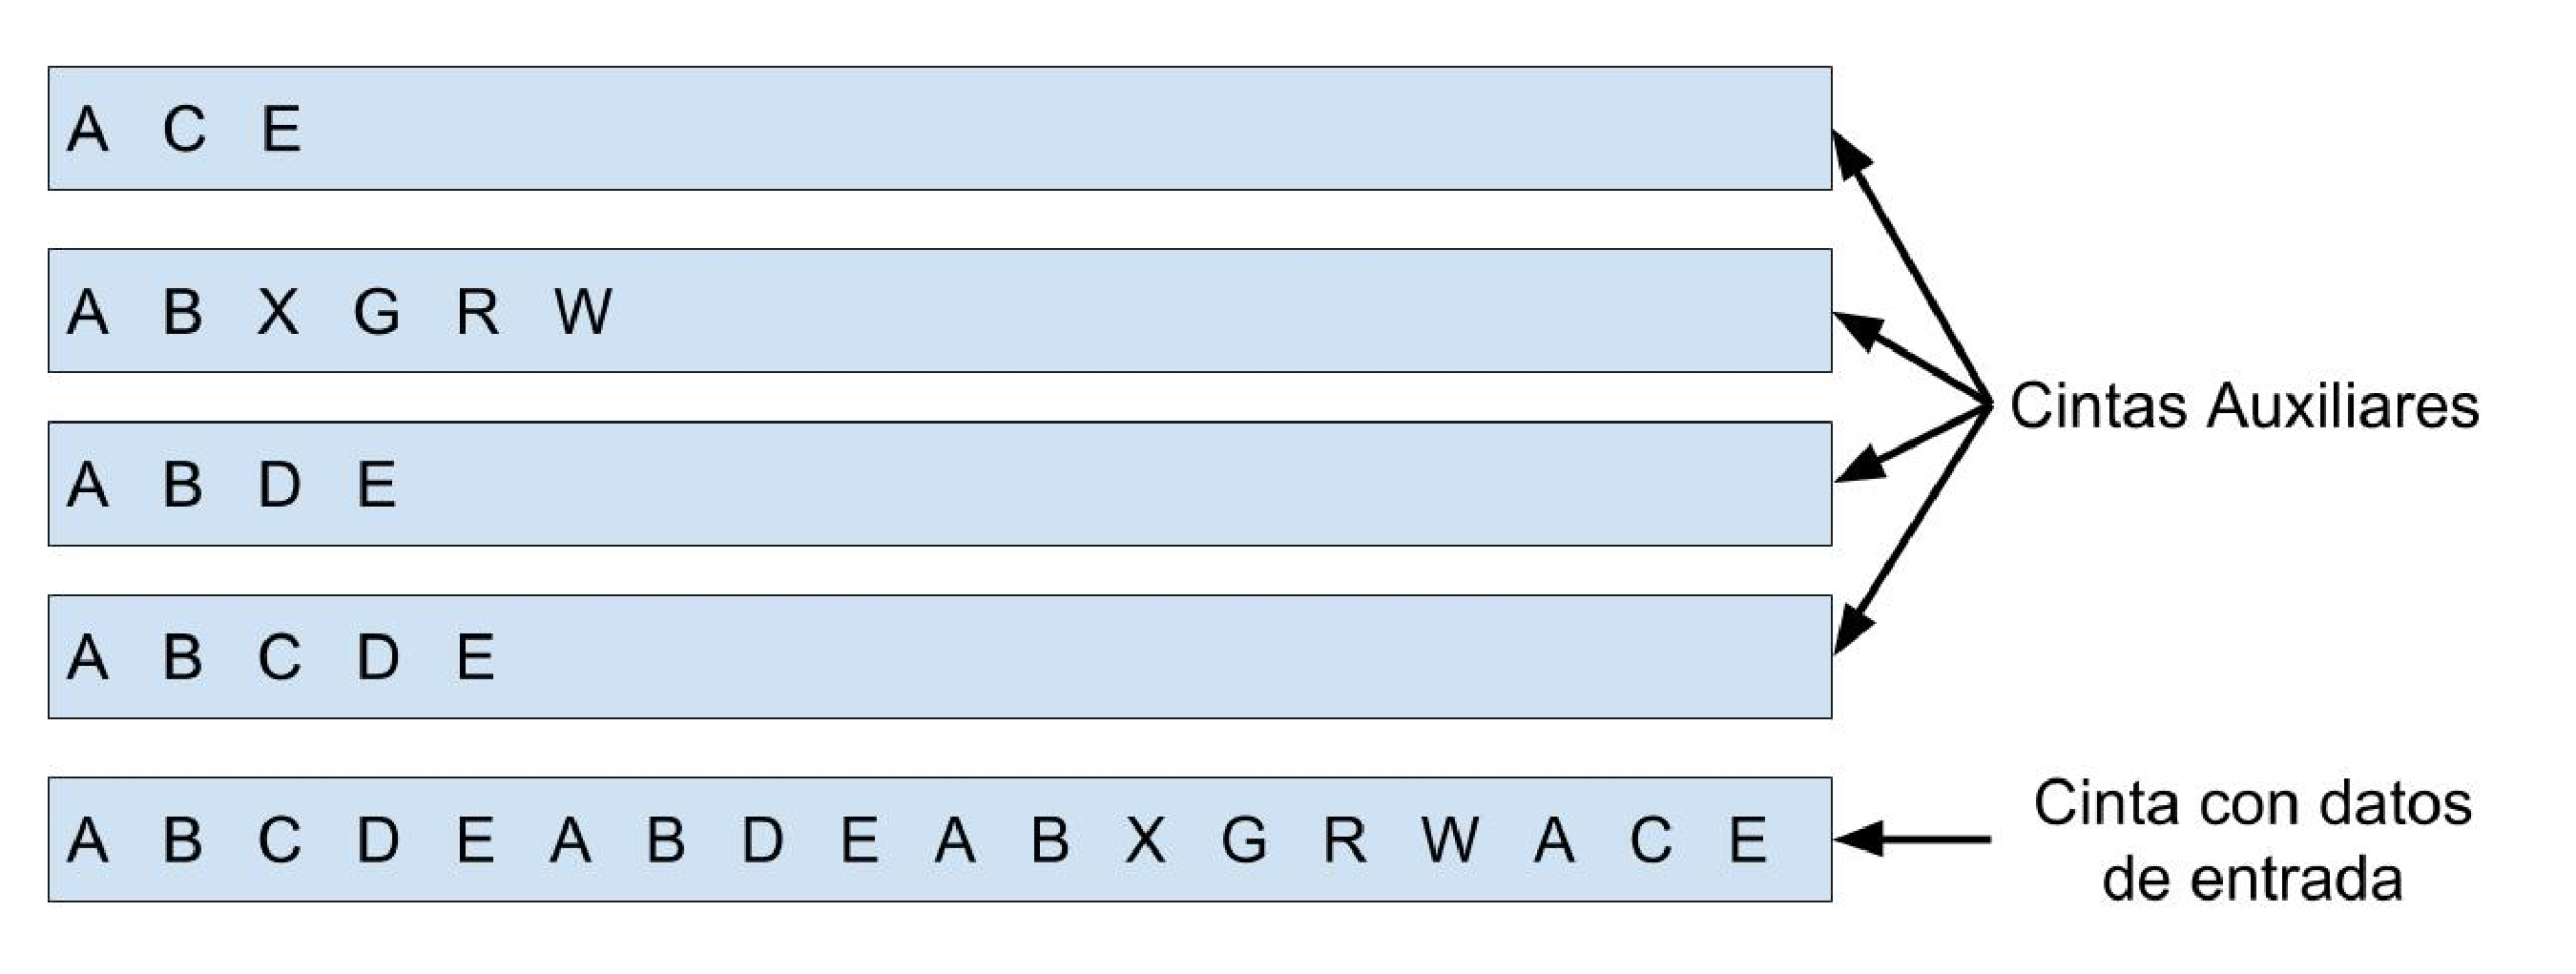
\includegraphics[width=1.0\columnwidth]{chap4/Imagenes/algoritmo1.eps}
\caption{Ejemplo del algoritmo con una m\'aquina de Turing multicinta.}
\label{fig:alg01}
\end{figure}
 